\documentclass[12pt,a4paper]{article}
\usepackage[utf8]{inputenc}
\usepackage{amsmath}
\usepackage{graphicx}
\usepackage{amsfonts}
\usepackage{amssymb}
\author{Drumea Alexandru-Daniel}

\title{Named Entity Recognition For The Romanian Language}
\begin{document}
\begin{titlepage}
   \begin{center}
		Universitatea "Alexandru Ioan Cuza" din Iași\\
       Facultatea de Informatică\\
  	\vspace{1cm}

   	
\includegraphics[scale=1]{fii}
  		       	
 	   \vspace{1cm}
		{\huge
       \textbf{Named Entity Recognition}
 
       \vspace{0.5cm}
        For The Romanian Language
 		}
       \vspace{3cm}
 
       \textbf{Drumea Alexandru-Daniel}\\
       \textbf{Sesiunea:} Iulie, 2019\\
		\textbf{Coordonator științific:} Prof.Dr. Cristea Dan
   \end{center}
\end{titlepage}

\tableofcontents
\newpage

\section{Introduction}

\subsection{Abstract}
	\qquad \quad Computer science is the study of processes that interact with large volumes of data, that can be represented in the form of programs. It enables the use of algorithms to manipulate, compute, store and communicate digital information. The above mentioned field is relatively new in the scientific community, as it employs the use of computers in order to ease human labour and aid in completing activities which otherwise would take significantly longer time to complete.
	
\qquad Such activities include natural language processing, a topic of research which is concerned with the interactions between computers and human (natural) language, in particular how to program computers to process and analyze large quantities of natural language data. One of the challenges in this field is “named entity recognition”, a topic of great research in modern times.

\qquad	Named entity recognition is a subtask of information extraction that seeks to locate and classify mentions of known named entities in unstructured texts into pre-defined categories, such as person names, organization names, geographical locations and miscellaneous such as date and time, geo-political relations etc.

\qquad	Presently, conferences such as CoNLL address the issues and challenges of the task of classifying named entities and award prizes for papers that have most contributed to perfecting human language analysis in general and NER in particular.

\qquad	The scientific community in this field has currently reached a high level precision and recall for much studied languages such as English and German. This can stand as a base level on which to place other more sophisticated technologies. 

\qquad	Techopedia, the leading online technical dictionary, explains “Named-entity recognition is a state-of-the-art intelligence system that works with nearly the efficiency of a human brain. NER systems are structured in such a way that they are capable of finding entity elements from raw data and can determine the categories to which the elements belong. The system reads the sentence and highlights the important entity elements in the text. A NER system might be made sensitive to different types of entities depending on the project. This means that the NER system designed for one project may not be reused for another task. Similarly, NER faces many challenges which include the extraction of correct information for specific but closely related categories". In addition to those previously stated, the problem of recognizing named entities may be broken down, conceptually, in two problems, which are the detection of names and classification of said names by the type of entity they refer to (e.g. person, organization, location and miscellaneous). 

\qquad	In order to evaluate the results of such systems, one must define the concepts of precision, recall and F-measure functions, as defined by academic conferences such as CoNLL.

\qquad	Precision is the number of predicted entity name spans that line up exactly with spans in the gold standard evaluation data. I.e. when [Person Hans] [Person Blick] is predicted but [Person Hans Blick] was required, precision for the predicted name is zero. Precision is then averaged over all predicted entity names. Recall represents the number of names in the gold standard that appear at exactly the same location in the predictions, while the F-measure (or the F1 function) is the harmonic mean of these two.

\qquad	The technology currently available for this type of information extraction is comprised of Python libraries and Java applications, which offer support for the aforementioned languages (German and English), with great F-measure scores. To describe the available resources for said languages, one needs to understand the Conditional Random Fields Classifiers, which are described Sutton and McCallum (2010) paper, “An Introduction to Conditional Random Fields” as follows “A solution(n.r Named entity recognition) to this problem is to model the conditional distribution \textit{p(y$|$x)} directly, which is all that is needed for classification. This is a conditional random field (CRF). CRFs are essentially a way of combining the advantages of classification and graphical modeling, combining the ability to compactly model multivariate data with the ability to leverage a large number of input features for prediction. The advantage to a conditional model is that dependencies that involve only variables in \textit{x} play no role in the conditional model, so that an accurate conditional model can have much simpler structure than a joint model”. A corpus is a large data set consisting of bodies of text, which are either annotated or not. Seen from the perspective of building a NER system, a corpus should include annotations of name entities, together with their classes, out of which a learning system can be trained to recognise name entities.

\qquad	Stanford NER is a Java implementation of a Named Entity Recognizer. Stanford NER is also known as a CRF Classifier. The software provides a general implementation of  the linear chain Conditional Random Field (Sutton \textit{et al}, 2011) sequence models. That is, by training ones own models on labeled data, one can actually use this code to build sequence models for NER or any other task. The English corpus is included in the Stanford NER package and will correctly tag above 90$\%$ of named entities.

\qquad	NLTK (Natural Language Toolkit) is a "Python package providing a series of natural language corpora and APIs of wide varieties of NLP algorithms and it works in three stages: word tokenization, part-of-speech tagging and named entity recognition"("Introduction to NER" article, 2018).

\qquad	SpaCy is a natural language processing library in Python, known for its industrial-strength classification capabilities. "SpaCy supports numerous entity types and can be trained on a multitude of languages from scratch"("Introduction to NER" article, 2018).

\qquad	All of the technological solutions above are benchmarks for either the independent, hobbist researcher or for the international community restlessly working to improve the processing of human language with the use of computers. However, even with a language-independent  approach, getting very good results on these platforms needs large quantities of training data, not easily achievable in languages having rather scarce annotated resources. Among these - Romanian, despite the fact that some offer multi-language and language-independent support.

\subsection{Motivation}

\qquad	\quad	The writer of this paper is highly motivated by the problem of creating a model of NER for the Romanian language, as it may serve as a template for other languages with Latin roots such as French, Spanish, Portuguese etc. The steps taken to achieve the task at hand include the use of the aforementioned technologies, in order to create a web application which provides one with statistics of the training process, pre-trained corpora as well as a classifier for unlabeled texts.	

\qquad In addition to the added flexibility of the topic and of the more nuanced variety of expressions, the Romanian language, being a much less known language than English benefits from a much smaller international research community to create models, gazetteers, training data, or named entity recognition software. The previous argument is to be added to the author's motivation to create a template for the aforementioned research community in the field of Natural Language Processing in general and Named Entity Recognition in particular.

\qquad NER models are used in a wide range of applications in the field of Natural Language processing and Information Retrieval. One such example is in automatically summarizing CVs, which consists of summarizing a CV, thus enabling Human Resources departments to quickly compile large volumes of personnel data. Running a NER model on a large collection of articles once and storing the entities associated with them permanently, would result in optimization of a search engine, which would not have to search the whole collection for the entered entity that occurs in a query each time a query is initiated. Another application of NER is simplifying customer support as it can be used in recognizing relevant entities in customer complaints and feedback such as Product specifications, department or company branch details, so that the feedback is classified accordingly and forwarded to the appropriate department responsible for the identified product.

\section{Theoretical Considerations, State-of-the-Art Technologies and Data Formats}
\subsection{Data Formats Used in the Current Thesis}
\qquad \quad This chapter describes a series of theoretical notations and the meta-data used in the process of named entity recognition. The files used contain specialized annotations used by the compiler in the categorization of the entities and prediction of their type.

\qquad The CoNLL-U Plus Format can encode any kind of annotation using a combination of the sentence-level comments and the MISC attributes, this format can have any number of non-zero columns, as well as a sentence-level comment (depicted by the use of $\#$ at the beginning of the line, used in order to either set a sentence id, or to write the sentence as raw text). This extends the CoNLL-U format which is widely used in Natural Language Processing, but is impractical in Named Entity Recognition due to its fixed number of columns (ten).

\qquad QuoVadis is a corpus displaying semantic relations in free text. As stated in the paper, "Developing a lexical-semantic knowledge base to be used in Natural Language Processing (NLP) applications is the main goal of the research described in this chapter (n.r. paper). Such resources are not available for many languages, mainly because of the high cost of their construction. The knowledge base is built in such a way as to facilitate the training of programs aiming to automatically recognize in text entities and semantic relations.[...] it includes annotations for the spans of text that display mentions of entities and relations, for the arguments (poles) of the relations, as well as for the relevant words or expressions that signal relations"(Cristea \textit{et al}, 2014). The data that comprises this corpus will be used in the training of the NER tagger this paper intents to build. The layers of annotation in the aforementioned corpus are as follows: segmentation at text level (marks the sentence boundaries in the raw book text), tokenization (demarcates words or word compounds, but also numbers, punctuation marks, abbreviations etc), part-of-speech tagging, lemmatization (determines lemmas of words) and noun-phrase chunking, which explores the previously generated data and adds information regarding noun phrase boundaries and their head words. In the scope of training the NER, the application to be presented in the following sections uses the part-of-speech tagging provided by the QuoVadis corpus, as well as the noun phrase chunking to create tab separated values (.tsv), a file to be trained by the Stanford CRF classifier. The data of the aforementioned corpus, which is initially comprized in an .xml type file, will be extracted and each "entity" tag will be added to the .tsv file, as highlited in Figure 1.

\begin{figure}[h!]
\begin{center}
  \makebox[\textwidth]{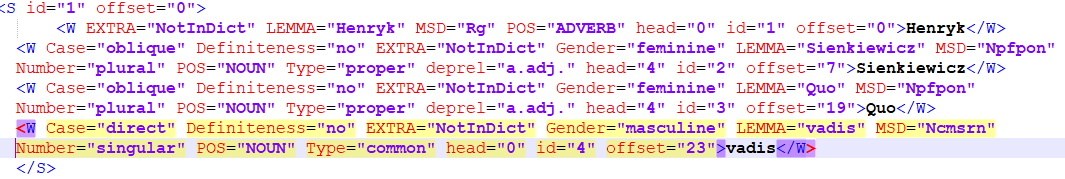
\includegraphics[width=\textwidth]{tempsnip} }
\end{center}
\caption{Data of the QuoVadis corpus}
\end{figure}

\qquad RONEC (Dumitrescu \textit{et al}, 2018) is a corpus of annotated data consisting of 5127 sentences, classified in 16 classes with a total of 26376 entities. It is used as a template for the training files, as well as for the named entity data it contains. From this file, the classificator will use the template of the file (CoNLL-UP format), as well as the data classified as person, organization, geographical location, or miscellaneous. The RONEC.conllup file is depicted in figure 2. 
\begin{figure}[h!]
\begin{center}
  \makebox[\textwidth]{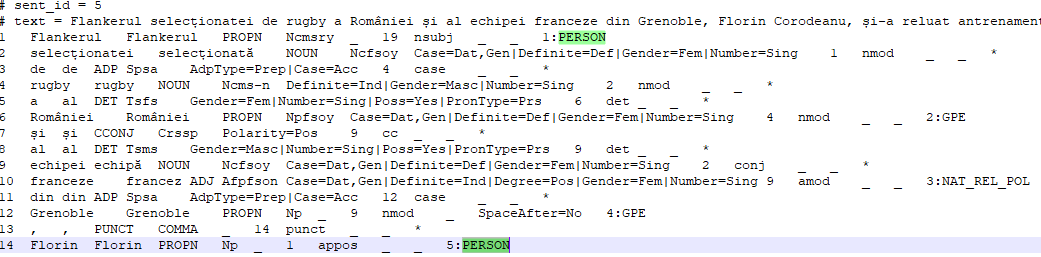
\includegraphics[width=\textwidth]{ronec} }
\end{center}
\caption{Data of the RONEC corpus}
\end{figure}

\qquad After the processing of the data in the two aforementioned corpora, the custom file to be used in the process of training, will consist of roughly 195000 entries, with their named entity recognition label, which is detailed below.
\begin{figure}[h!]
\begin{center}
  \makebox[\textwidth]{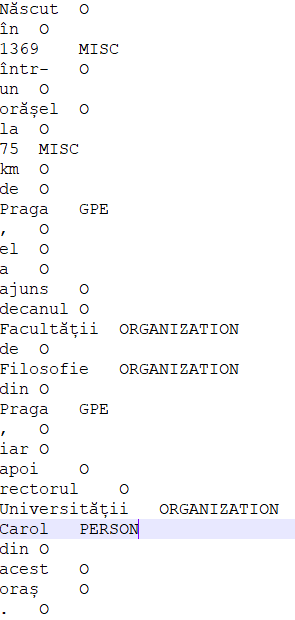
\includegraphics[scale=0.5]{processed} }
\end{center}
\caption{Data of the processed corpus}
\end{figure}

\qquad In Figure 3, one can observe the form of the processed corpus is of the form entity <TAB> type. The types of entities are: person, organization, o (others, which describes an entity which is not a named one), GPE which depicts countries, cities, states, as well as MISC, which will cover geo-politic entities, date and time, facilities and works of art.
\subsection{Deploying Web Applications Using Python}

\qquad \quad As the result of the application of the theoretical considerations and algorithms presented in this thesis will be comprised in a web application, it is very important to note some of the frameworks and libraries to be used.

\qquad One of the applications which provide one with the best ease of use is called Flask.

\qquad Flask is a microframework for Python, that comes with built-in development, server and debugger, integrated unit testing support, RESTful request dispatching, is Unicode based, and is extensively documented.

\qquad A use-case of this framework is depicted in the figure below.

\begin{figure}[h!]
\begin{center}
  \makebox[\textwidth]{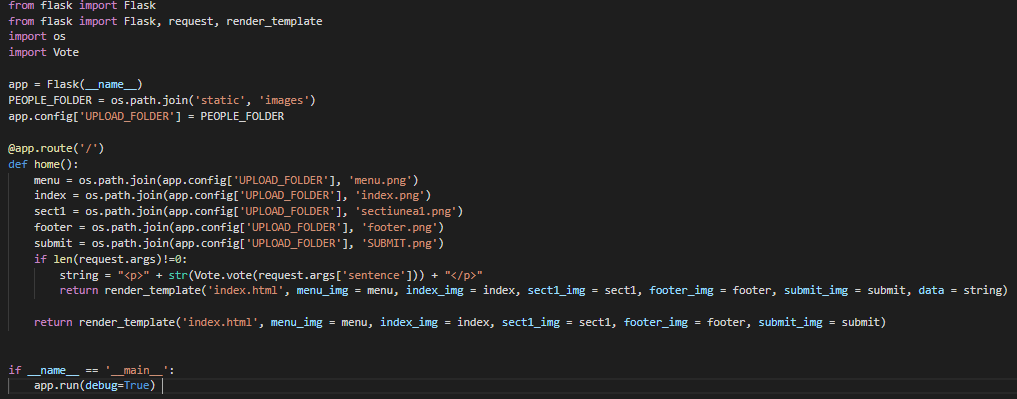
\includegraphics[scale=0.5]{flask} }
\end{center}

\end{figure}

\qquad The aforementioned use-case is as follows: a page that consists of three elements, a navigation bar, contents and the footer respectively. To be noted is that the page will present in the content section of its body a text-box in which the user will insert a sentence that will be sent to the server, the server catching that will execute a Python function using the parameters of the request. Finally, the server will use the results of said Python function and will alter the front-end accordingly.


\subsection{The Stanford Named Entity Recognition Software (Sutton \textit{et al}, 2015)}
\subsubsection{The Conditional Random Field Algorithm, Theoretical Considerations of the Stanford Software} 
\qquad \quad It is denoted as \textit{x = (x\textsubscript{1}, ..., x\textsubscript{n})} as the input sequence, i.e. the words of a sentence and \textit{ s = (s\textsubscript{1}, ..., s\textsubscript{n})} the sequence of output states i.e. the named entity tags. In conditional random fields, the conditional probability \textit{p(x\textsubscript{1}, ..., x\textsubscript{n}$|$ s\textsubscript{1}, ..., s\textsubscript{n})} is modeled. This feat is accomplished by defining a feature map function $\Phi$(x\textsubscript{1}, ..., x\textsubscript{n}, s\textsubscript{1}, ..., s\textsubscript{n}) $\in$ R\textsuperscript{d}, this maps the input sequence \textit{x} paired with an entire state sequence \textit{s} to some d-dimensional vector. Then one can model the probability as a log-linear model with the parameter vector $\omega$ $\in$ R\textsuperscript{d}: \[p(s|x; \omega) = \frac{exp(\omega \cdot \Phi(x, s))}{\sum_{s'}^{} exp(\omega \cdot \Phi(x, s'))},\] where s' ranges over all possible output sequences. For the estimation of $\omega$, it is assumed there is a set of n labeled examples {(x\textsuperscript{i}, s\textsuperscript{i})}, where i ranges between 1 and n. Now, the log-likelihood function is computed: 
\[\sum_{i=1}^{n} log( p(s\textsuperscript{i}|x\textsuperscript{i}, \omega))\]
The parameter vector $\omega$* is then estimated as:
\[\omega\textsuperscript{*} = argmax \textsubscript{$\omega$$\in$R\textsuperscript{d}} L(\omega)\]
The statement above means that each sequence will be tagged with the tagging associated with the highest probability. 

Now, the most likely tagging of a sentence x may be computed as:

\[s\textsuperscript{*} = argmax\textsubscript{s}p(s|x, \omega\textsuperscript{*})\]

\qquad Having understood the aforementioned algorithm, one may apply said algorithm both for part-of-speech tagging, as well as for named entity recognition. This algorithm is most prominently used by the Stanford NLP team as the nucleus for their named entity recognition software, on which this thesis has based its research into NER tagging in the Romanian language.
\subsubsection{The Operation of the Stanford Named Entity Recognition Software}

\qquad \quad This model uses the Conditional Random Field Algorithm in order to predict the features of an unknown word. 

\qquad All word features are stored in a window, that being comprised of the current word, previous word, next word, as well as orthographic features such as capitalization and overall form of a word (Jenny is generically depicted as Xxxxx, while AH1-N1 as XX$\#$-X$\#$). Additionally, features of high importance are also stored, features such as prefixes and suffixes, which are also stored in a window (Jenny is depicted as $<$Jen, $<$...ny$>$ $>$), as well as label sequences as feature conjunctions.

\qquad This method of recognition also employs the use of the Distributional Similarity Features on a large unannotated corpus, which will provide context of named entities, which will then be clustered on how similar their distributions are within the corpus in order to combat sparsity.

\qquad The Stanford Named Entity Recognition Software is highly used in the academical due to its multi-language and language-independent support, as well as to its speed and its open-source availability.
\subsection{The SpaCy Entity Recognition Module}
\qquad \quad SpaCy is a free, open source library that has made Natural Language Processing (NLP) much simpler in Python.

\qquad It provides users with a statistical system which is highly efficient for named entity recognition, which can assign labels to groups of tokens which are contiguous. It can accurately recognize a wide variety of named entities or numerical entities, and can enable the addition of arbitrary classes to the model, by training it to enable bespoke examples. 

\qquad Because this program is widely used in the industry, the company has not yet provided many technical specifications, other than it uses convolutional neural networks (CNN).

\qquad A convolutional neural network is a class of deep neural networks, which are used in a wide variety of tasks in deep learning, ranging from analyzing visual imagery, to sentence classification and named entity recognition. 

\qquad "Convolutional neural networks (CNN) utilize layers with convolving filters that are applied to local features"(Kalchbrenner \textit{et al}, 2014). Originally invented for computer vision, CNN models have subsequently been shown to be effective for NLP and have achieved excellent results in semantic parsing (Yih \textit{et al}, 2014), sentence modeling (Liu \textit{et al}, 2015), and other traditional NLP tasks. 

\qquad Convolutional Neural Networks are used in Natural Language Processing in general and Named Entity Recognition in particular because of their ability to extract features. These networks are applied to embedding vectors of a given sentence with the aim of extracting useful features such as relationships between words that are closer together in a sentence, or the relation between sentences. Moreover, Convolutional Neural Networks will capture the relationships and general meanings of a sentence, which also represents an important advantage for good classification.

\qquad The use of CNNs in NER is very similar to their use in image classification. Given a sequence of words \textit{w\textsubscript{1:n} = \textit{w\textsubscript{1},…,w\textsubscript{n}}}, where each is associated with an embedding vector of dimension \textit{d}.

\qquad A 1D convolution of width-\textit{k} is the result of moving a sliding-window of size \textit{k} over the sentence, and applying the same convolution filter or kernel to each window in the sequence, i.e., a dot-product between the concatenation of the embedding vectors in a given window and a weight vector \textit{u}, which is then followed by a non-linear activation function \textit{g}.

\qquad Considering a window of words \textit{w\textsubscript{i},…,w\textsubscript{i+k}}, the concatenated vector of the \textit{i}th window is then:

\[x\textsubscript{i} = [w\textsubscript{i}, ,w\textsubscript{i+1},…,w\textsubscript{i+k}] \in R\textsuperscript{k $\cdot$ d}\]

The convolution filter is applied to each window, resulting in scalar values \textit{r\textsubscript{i}}, each for the \textit{i}th window:

\[r\textsubscript{i} = g(x\textsubscript{i} \cdot u) \in R\]

As previously stated in this thesis, SpaCy is an industrial-strength classifier, meaning that it is currently used by companies in order to achieve different tasks of a large scope, tasks which include product management, human resource management as well or search engine tuning. According to the lead-developer of SpaCy, companies such as Airbnb (which is an accomodation booking company), Quora (an online technology forum) or Allen Institute for Artificial Intelligence currently employ this software to extend and improve their services. 

\subsection{The Theoretical Foundations of the Gazetteer Method in Named Entity Recognition}

\subsubsection{The Brute Force Method}
\qquad \quad The first step in implementing this method implies the creation of a different list of items for each entity one desires to recognize, on which search operations will be applied in a later step in order to classify names.

\qquad Secondly, a large corpus of data needs to be appended to each list in order to achieve a great level of precision and recall for each of the named entities.

\qquad This method is quite restrictive due to the difficulties of comprising a corpus large enough to accomodate the varieties of named entities one may encounter, as well as the difficulties in keeping it up to date automatically. Moreover, the ambiguity resolution factor (the interpretation of metaphors, entities of the same name etc) is rather low, a fact which also leads to low precision.

\qquad Despite its disadvantages, the Gazetteer Method is a highly powerful method in named entity recognition, due to its speed, ease of manual improvement and relative ease of use.

\subsubsection{Improving the Brute Force Method}

\qquad \quad In order to improve the method presented in the previous subsection, one must use a part-of-speech tagger as to extract only words that are proper nouns, thus optimizing the speed of the search algorithm and improve the overall performance. After having taken these steps, the search algorithm may be applied on each proper noun which is an output of the part-of-speech tagger.

\quad To achieve those previously stated, the application presented in this thesis uses a part of the Stanford NER model, the Stanford POS Tagger. This tool applies the Conditional Random Field algorithm on the set of untagged data for obtaining the Part-Of-Speech Tagging necessary. The input data for the POS Tagger is comprised of a Romanian language model available on the Stanford platform, said model containing over 125000 tagged parts of speech.

\subsection{State-of-the-Art Methods with Respect to The Romanian Language}

\qquad \quad The aforementioned methods of tagging named entities are widely used by companies and researchers alike, being highly appreciated for their reliability and overall correctness. They have proved to produce good F-measure score in languages which are highly restrictive with respect to the topic of the sentence.

\qquad For example, in English, one may represent a noun-phrase by the following regular expression:
\[pattern = 'NP: {<DT>?<JJ>*<NN>}',\]
in which NP depicts noun-phrase, DT is a determiner, JJ an adjective and NN a noun. The previously stated regular expression translates as: a noun phrase, NP, should be formed whenever the chunker finds an optional determiner, DT, followed by any number of adjectives, JJ, and then a noun, NN. One needs a noun phrase in order to more efficiently classify words as chunks, as well as to get a better understanding of the context and reduce the number of entities to be classified. For example in the following sentence: \textit{"Google, the giant American company, has been fined $\$$5.1 billion dolars."}, the chunk "the giant American company" is a noun phrase which will offer the named entity recognition software the context needed to classify Google as an organization.

\qquad Meanwhile, in the Romanian language, the above stated sentence may be translated as \textit{"Google, giganta companie americana, a fost amendata cu 5.1 miliarde de dolari."}, which is a natural context having a natural topic of the sentence. One may observe that the order in which the adjectives are placed is highly flexible, ranging from the above stated $<$DT$>?<$JJ$>*<$NN$><$JJ$>*$ to $<$DT$>?<$NN$><$JJ$>*$("compania giganta americana"), a fact which is much harder to represent using regular expressions because there exist much more variations in the topic of a sentence rather than in English.
\section{The Romanian Named Entity Recognition Software}

\qquad \quad The object of the current thesis is to combine the three methods described in the previous chapter in a reliable and fast Named Entity Recognition Software for the Romanian language in the form of a web application.

\qquad The resources that will be used are to be detailed and exemplified in the current chapter, as well as the application logic and the results of the processing.

\subsection{Data Preprocessing}

\qquad \quad In order to obtain fast, reliable data, the corpora described in the the first section of the previous chapter in the current thesis has to be preprocessed in order to obtain a ConLL-UP formatted file, the one that is needed for the training of the customly-built named entity tagger described in this thesis.

\qquad Firstly, one has to extract the relevant data from the RONEC file, in order to comprise the training file for the Stanford NER software. This feat is to be accomplished by making use of the Python script in Figure 4.
\begin{figure}[h!]
\begin{center}
  \makebox[\textwidth]{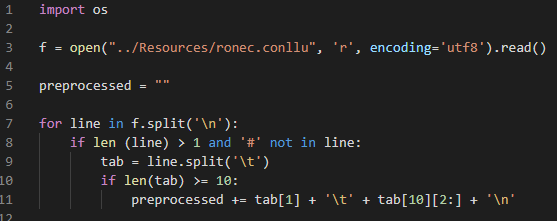
\includegraphics[width=\textwidth]{preprocess} }
\end{center}
\caption{Preprocessing the RONEC corpus}
\end{figure}
After data has been processed, the ronec.conllu is presented as in Figure 5.
\begin{figure}[h!]
\begin{center}
  \makebox[\textwidth]{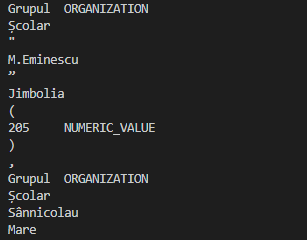
\includegraphics[scale = 1]{output} }
\end{center}
\caption{Output of the Python Script in Figure 4.}
\end{figure}

\qquad One may notice that the shape of the file to be used for training is not ideal at this point, as there are words without tagging, mainly those that are parts of noun phrases. In the interest of simplicity, the following Python script will be used in order to complete the file with the missing tags. One is inclined to see that if between two tagged words there are words which are not tagged, there is a high probability that the words between the two tags are of the same tag as the former. Errors are insignificant to the training, as the corpus contains 120000 entries.

\qquad This script will loop 500 times to ensure that the Romanian corpus is complete and contains no white spaces in the column assigned to the named entity type. This procedure is described in Figure 6.

\begin{figure}[h!]
\begin{center}
  \makebox[\textwidth]{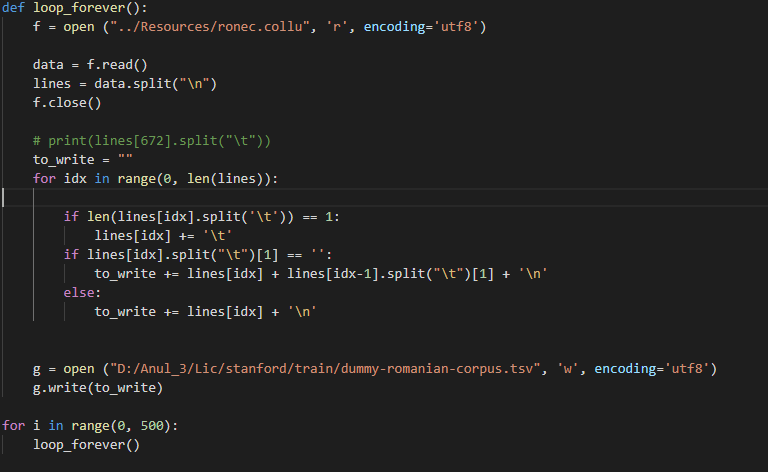
\includegraphics[scale = 0.8]{completion} }
 
\caption{Completing the types of the entities which are part of noun phrases.}
\end{center}

\end{figure}

\begin{figure}[h!]
\begin{center}
  \makebox[\textwidth]{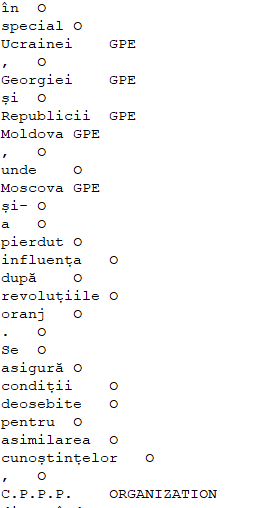
\includegraphics[scale = 0.55]{preview_dummy} }
\end{center}
\caption{The output of the Python script in Figure 6.}
\end{figure}

\qquad One may proceed with the extraction of data from the QuoVadis corpus, with the mention that a python xml parser will be needed to extract the words containing the tag $<$entity$></$entity$>$, as well as to extract the "Type" attribute and the text of the entry in the .xml file.

\begin{figure}[h!]
\begin{center}
  \makebox[\textwidth]{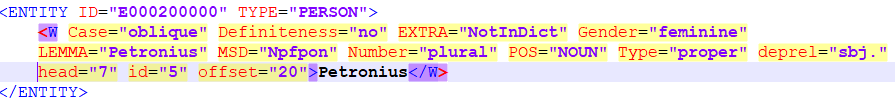
\includegraphics[width=\textwidth]{entity} }
\end{center}
\caption{The exemplification of an "entity" type entry in the QuoVadis corpus.}
\end{figure}

\qquad In the aftermath of those above, a complete and comprehensive training file is comprised and ready to serve both as a gazetteer and an input for the Conditional
Random Field classification algorithm.

\subsection{Stanford Named Entity Recognition Method}

\qquad \quad Having comprised the training data, one is ready to apply the Stanford NER, by far the most reliable Natural Language Processing library on the market. The aforementioned package is written in Java, so one will need a proper Java Development Kit installed in order to run it.

\qquad Having prepared the environment needed, one needs to load the Stanford NER engine, available online for free for academic purposes. 

\qquad The classification file compiled at the previous step (Subsection 3.1 Data Preprocessing) will now serve as a training file in the context of the program itself, as well as the two vectors (\textit{x} - word vector, \textit{s} - state vector) presented in Subsection 2.1.1 - "The Conditional Random Field Algorithm, Theoretical Considerations of the Stanford Software", the respective file is to be placed in the folder $"./$train$"$ of the home folder of the Stanford classifier software. Moreover, the classifier software needs to be given a list of proprieties, most of which are fixed for the Named Entity Recognition, some of which may be changed. Said proprieties are presented in Figure 9.

\qquad The trainFile field represents the location of the .tsv (tab separated variables) file presented in Section 2.0.1 and built at the previous section, serializeTo field is the location to which the serialized, trained file will be written, while the map field is the exact layout of the columns of the .tsv file, in this case the numbering of the columns will start from 0, the first column being named as "word", whilst the second column (1) will be named as "answer", meaning the type of the named entity. It is important to note that the first column will be the vector of x (words) in the Conditional Random Field Algorithm (Subsection 2.1.1), while the second will be the vector of s (states) in the same algorithm.
\begin{figure}[h!]
\begin{center}
  \makebox[\textwidth]{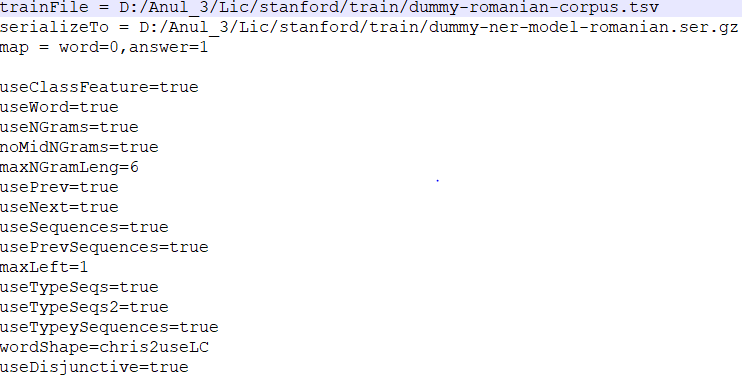
\includegraphics[width=\textwidth]{StanfordNER} }
\end{center}
\caption{The list of proprieties of the Stanford NER.}
\end{figure}

\qquad Having set the proprieties, one has to run the command in Figure 10 in the home folder of his Stanford NER software.

\begin{figure}[h!]
\begin{center}
  \makebox[\textwidth]{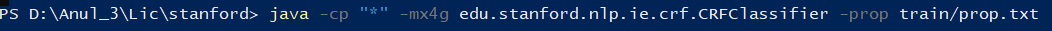
\includegraphics[width=\textwidth]{command} }
\end{center}
\caption{The command to run the Stanford Trainer.}
\end{figure}

\qquad Having run the command, the training will output the serialized, trained file, having applied the Conditional Random Field Classifier on all the windows it produced for over 100 iterations. The training process is time and memory consuming. For the latter, one may observe that the fourth parameter of the command in Figure 10 is the memory allocated for the training process (in the current case 4 GB of memory have been allocated). 

\qquad In Figure 11, the training time for 5000 data entries is presented, which is around 6 minutes, the training having been done after 131 iterations and will produce satisfying results at tagging level. However, for a higher F-measure score, this thesis will use all of the pretrained data that has been comprised at the previous subsection, adding up to 195000 entries.

\begin{figure}[h!]
\begin{center}
  \makebox[\textwidth]{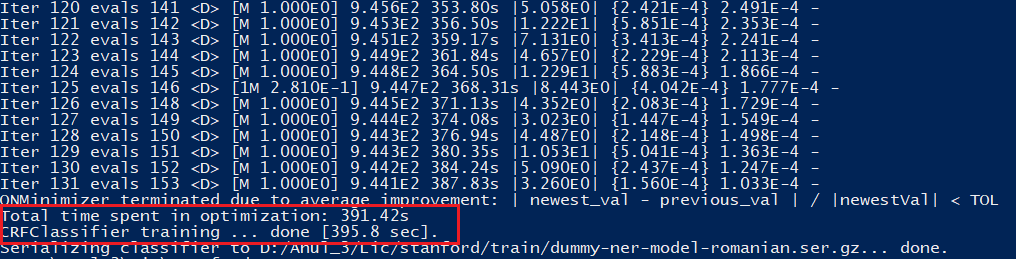
\includegraphics[width=\textwidth]{Classifier20000} }
\end{center}
\caption{Result for 5000 entries.}
\end{figure}

\qquad In order to run the classifier on all 195000 entries, various tweaks had to be made to the training file, such as the removal of some irrelevant punctuation (such as "():,"), because otherwise the Java stack would be exceeded. 

\begin{figure}[h!]
\begin{center}
  \makebox[\textwidth]{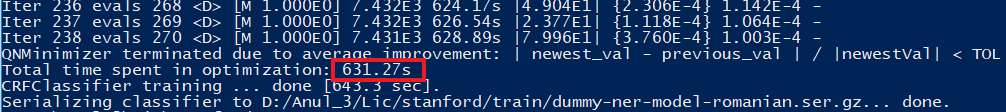
\includegraphics[width=\textwidth]{Classifierall} }
\end{center}
\caption{Result for all 195000 entries.}
\end{figure}


\qquad In order to run the now-trained classifier on raw, unannotated data, one must implement a Python script, using the StanfordNERTagger class of the NLTK (Natural Language Toolkit) Python library this thesis has mentioned in the Introduction section.

\qquad An example of such Python script is presented in Figure 13, this exact script will be used in the web application this thesis aims to implement. Moreover, in Figure 14, one notices the results of a tagging example for the purpose of visualizing the results. These results are to be used as data for the Statistics section of this thesis, where one will be introduced to the numerical facts of this classification, compared to the other two that will be presented in the following subsections.

\begin{figure}[h!]
\begin{center}
  \makebox[\textwidth]{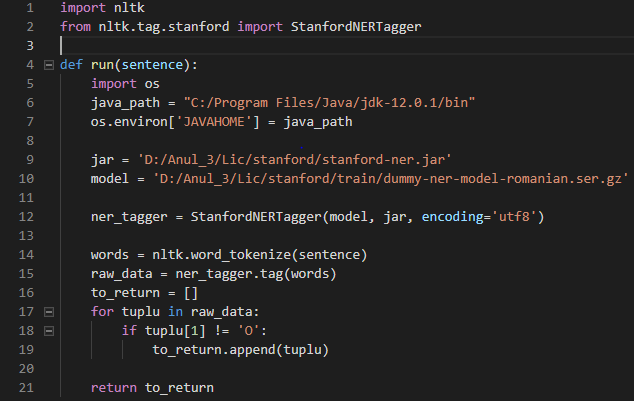
\includegraphics[width=\textwidth]{stanfordtrained} }
\end{center}
\caption{Example of Python script to run the trained classifier.}
\end{figure}

\begin{figure}[h!]
\begin{center}
  \makebox[\textwidth]{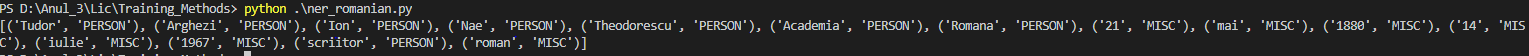
\includegraphics[width=\textwidth]{ouptut1} }
\end{center}
\caption{Output of the Classifier.}
\end{figure}

\qquad One may notice that the output of the classification in this case is a list of tuples having the following format [(word$\_$text1, NER$\_$tag1),(word$\_$text2, NER$\_$tag2), ..., (word$\_$textn, NER$\_$tagn)]. This format is the one to be used in the manual training of the test data used in the Statistics section of the application, as well as for the other classifiers.

\subsection{The Practical Application of the Gazetteer Method}
\subsubsection{Creation of the List of Entities}

\qquad \quad The creation of this corpus is highly time consuming. The internet is the best resource as to gain as much information as possible in order to complete the list necessary for a satisfactory classification of some more complex sentences.

\qquad Data from the Wikipedia article dedicated to Romanian surnames have been extracted, a list of the most common 2000 first names in the language, as well as data from the previously presented RONEC and QuoVadis corpora have been extracted in order to comprise the "PERSON.txt" file for named entities of this particular types. The same procedure has been applied for the other 3 categories of named entities (ORGANIZATION, MISC, GPE), with the mention that for the geographical entities, data has also been extracted from the gazetteer comprised in the study "A Mixed Approach in Recognising Geographical Entities in Texts"(Cristea \textit{et al}, 2015).

\qquad The format of the above mentioned files is one-per-line in a simple text file, for easier access and reduced complexity of the search algorithm. Figure 15 depicts a snippet of the "PERSON.txt" file, comprising of 43727 entries.

\begin{figure}[h!]
\begin{center}
  \makebox[\textwidth]{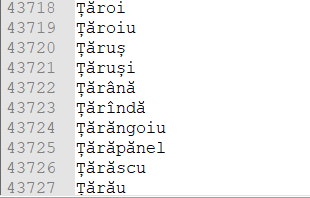
\includegraphics[scale=1]{PERSON} }
\end{center}
\caption{Snippet of the PERSON.txt file.}
\end{figure}

\subsubsection{The Operation of the Gazetteer Method}

\qquad \quad First and foremost, one must run the Stanford POS Tagger in order to appropriately tag the parts of speech in the given test text. The code of said tagging is depicted in Figure 16, while the output in Figure 17. The test data to which the tagger is applied is the sentence: \textit{"Tudor Arghezi, pseudonimul lui Ion Nae Theodorescu, Academia Romana, nascut la 21 mai 1880, Bucuresti decedat in 14 iulie 1967 a fost un scriitor român, cunoscut pentru contribuția sa la dezvoltarea liricii românești sub influența baudelairianismului. Opera sa poetică, de o originalitate exemplară, reprezintă o altă vârstă marcantă a literaturii române. A scris, între altele, teatru, proză (notabile fiind romanele Cimitirul Buna Vestire și Ochii Maicii Domnului), pamflete, precum și literatură pentru copii. A fost printre autorii cei mai contestați din întreaga literatură română".}

 \begin{figure}[h!]
\begin{center}
  \makebox[\textwidth]{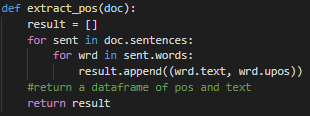
\includegraphics[scale = 1]{POSprogram} }
\end{center}
\caption{The function for the Part of Speech Tagger.}
\end{figure}

\begin{figure}[h!]
\begin{center}
  \makebox[\textwidth]{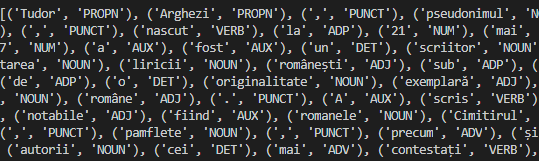
\includegraphics[scale = 1]{outputPOS} }
\end{center}
\caption{A snippet of the output, when run on test data.}
\end{figure}

\qquad As the gazetteer method usually is insensitive to the context, which means that it sees the words in a sentence as a list, one may filter the results presented above and extract only said words that are nouns and proper nouns, and then proceed to the tagging itself, with the returned result being of the same type as that of the one outputted by the classifier in the previous section. These facts are depicted in Figures 18 and 19.

\begin{figure}[h!]
\begin{center}
  \makebox[\textwidth]{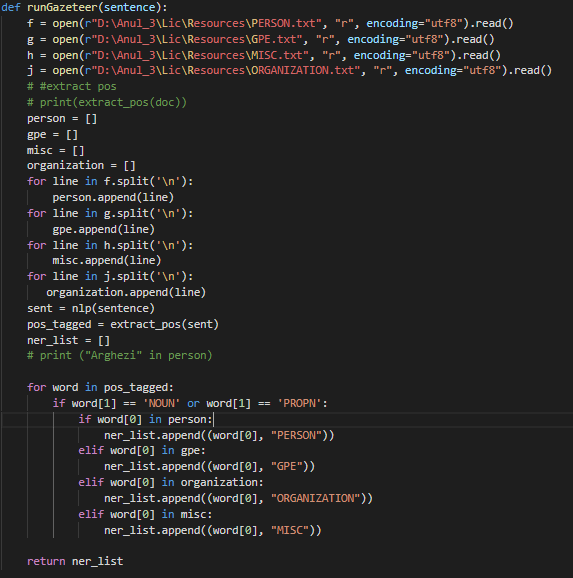
\includegraphics[width=\textwidth]{gazetteer} }
\end{center}
\caption{The function for the classification of the proper nouns.}
\end{figure}

\qquad One may see that the proper nouns that describe persons have been correctly classified, as well as those describing geographical location, meanwhile those describing miscellaneous named entities or organizations named entities, due to the vast scope of their respective entities are not perfectly recognized.

\begin{figure}[h!]
\begin{center}
  \makebox[\textwidth]{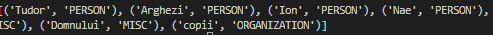
\includegraphics[scale = 1]{outputgazeteer} }
\end{center}
\caption{A snippet of the output when run on test data.}
\end{figure}

\subsection{SpaCy Named Entity Recogniser}

\qquad \quad In order to run the SpaCy software on a language that does not have any pretrained model, one needs to download the multi language model available on the SpaCy website in order to access data extracted from various Wikipedia pages, comprised into a training data set for the convolutional neural network (described in Subsection 2.2). The aforementioned model supports identification of PERSON, GPE, ORGANIZATION and MISC entities, similar to the other two methods described in the previous chapters.

\qquad Having downloaded the resources necessary for the execution, one has to import and load the model into the memory, as described in Figure 20.

\begin{figure}[h!]
\begin{center}
  \makebox[\textwidth]{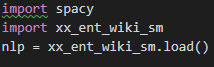
\includegraphics[scale = 1]{spacyimports} }
\end{center}
\caption{SpaCy imports}
\end{figure}

\qquad The SpaCy NER tagger will then work automatically, tagging the instances, the output being formatted to the format used in the previous two sections of the thesis (list of tuples of the form (word, entity), where entity is one of PERSON, ORGANIZATION, GPE or MISC). The execution of the SpaCy tagger is shown in Figure 21, while the output is in Figure 22, the input data being the same sentence as the aforementioned two other methods of classification.

\begin{figure}[h!]
\begin{center}
  \makebox[\textwidth]{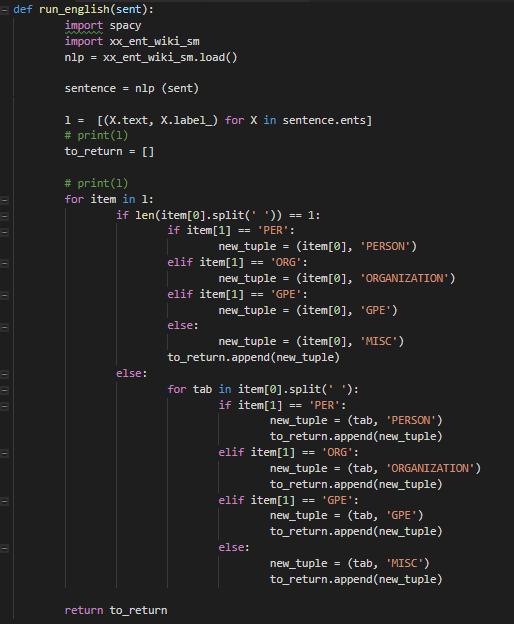
\includegraphics[width=\textwidth]{spacy_program} }
\end{center}
\caption{SpaCy execution and formatting the data.}
\end{figure}

\qquad It is to be observed that the classification is correct to a certain degree and becomes satisfying when taking into account that this classifier has no specific model for the Romanian language.

\begin{figure}[h!]
\begin{center}
  \makebox[\textwidth]{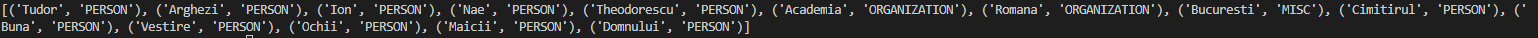
\includegraphics[width=\textwidth]{output_spacy} }
\end{center}
\caption{SpaCy results}
\end{figure}





\subsection{Statistics}

\qquad \quad In order to achieve comprehensive statistics, one must run the three aforementioned methods of classification on multiple examples from different spheres and contexts. For doing so, a list of 20 pieces of text has been comprised, the contents of which varying from scientific text, journalistic text, social media, academic or online article. 

\qquad The format chosen for this collection of data is a dictionary with two keys, the 'raw' tab, and the 'tagged' tab, with the raw tab containing the text as it is, unannotated, while the tagged tab contains the Named Entity Recognition done manually by the author. Figure 23 presents a snippet of the file mentioned above.

\begin{figure}[h!]
\begin{center}
  \makebox[\textwidth]{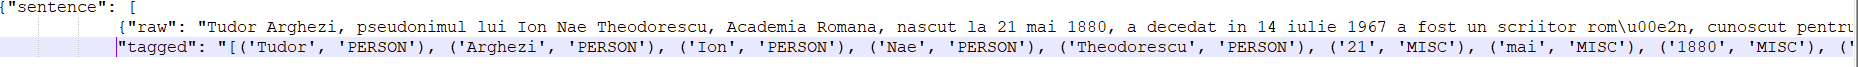
\includegraphics[width=\textwidth]{dictionary} }
\end{center}
\caption{Dictionary of test data.}
\end{figure}

\qquad In order to present the precision and recall functions, one must define some key terms.

\qquad The first of those is the term of true positive. One calls a word a true positive, if the word is a named entity, the classifier tagged the word as a named entity, and the category attributed the word is correct.

\qquad Secondly, one calls a false positive a word which is not a named entity, but has been classified as such.

\qquad Thirdly, a false negative is a either a named entity which has not been classified at all, or one which has been wrongly classified.

\qquad Lastly, a true negative is a word that is neither a named entity, nor has it been classified as such.

\qquad One computes the following metrics, which have theoretically addressed in Section 1 of the current thesis, for calculating the performance of each classifier:

\begin{enumerate}
\item \[precision = \frac{true\_positives}{true\_positives + false\_positives}\]
\item \[recall = \frac{true\_positives}{true\_positives + false\_negatives}\]
\item \[F-measure = 2 \cdot \frac{precision \cdot recall}{precision + recall}\]
\end{enumerate}

\qquad Each of these three metrics are relevant to the overall performance of one's Named Entity Recognition software. In this current thesis we address all 3 of them in order to asses the level of corectness each method of classification previously described achieves.

\qquad For each of the methods, one will compute a function in order to compute the parameters previously stated, as in the example in Figure 24.

\begin{figure}[h!]
\begin{center}
  \makebox[\textwidth]{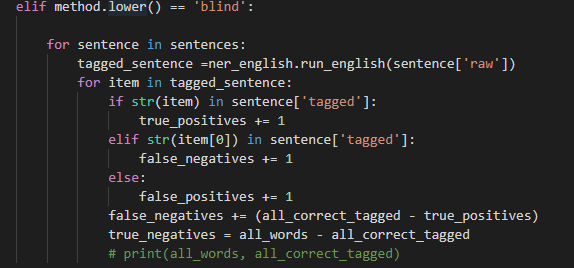
\includegraphics[width=\textwidth]{spacy_stats} }
\end{center}
\caption{The statistics function for the SpaCy method.}
\end{figure}

\qquad It is highly important to mention that variables "all$\_$words" and "all$\_$correct$\_$tagged" have been previously computed, the former being the sum of all words in the test examples (be them named entities or not), while the latter the sum of all manually tagged words (all of the named entities).

\qquad The result of these calculations is an excellent indicator to how the system performs, and which of the methods is better on this particular data set.

\qquad Figure 25 depicts the output of the precision algorithm presented above, similarly, Figures 26 and 27 present the output of the recall and F-measure algorithms respectively.

\begin{figure}[h!]
\begin{center}
  \makebox[\textwidth]{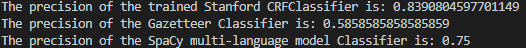
\includegraphics[width=\textwidth]{precision} }
\end{center}
\caption{The output of the precision algorithm.}
\end{figure}

\begin{figure}[h!]
\begin{center}
  \makebox[\textwidth]{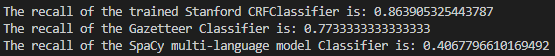
\includegraphics[width=\textwidth]{recall} }
\end{center}
\caption{The output of the recall algorithm.}
\end{figure}

\begin{figure}[h!]
\begin{center}
  \makebox[\textwidth]{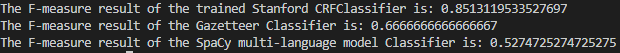
\includegraphics[width=\textwidth]{fmeasure} }
\end{center}
\caption{The output of the F-measure algorithm.}
\end{figure}

\qquad One must note that the results are bounded by 1 (it being the maximum precision, recall and F-measure achievable). If we were to scale the result to percentages, the most exact overall classifier (the metric of choice is the F-measure score), would be the trained Stanford Conditional Random Field Classifier, which has been previously presented in Subsection 2.1 from a theoretical standpoint and in Subsection 3.2 from a practical standpoint.

\qquad The results show that inevitably the best classifier is, with a score of 85.1$\%$ is the trained Stanford classifier, while the least accurate is the SpaCy, an expected result, due to its lack of Romanian language-specific models. 

\qquad The lack of higher accuracy in the context of the Gazetteer method is due to its lack of context data, as well as due to the lack of sufficient data in order to interpret different ORGANIZATION and MISC entities, despite the relatively high number of instances present in the training data.

\subsection{The Voting Function}

\qquad \quad In order for the application to achieve the best possible classification comprised of the three methods, one must implement a voting system in order to best choose the classification needed for the untagged sentence.

\qquad This thesis proposes a voting function which combines the F-measure results computed in the previous subsection, making each of the F-measure scores ratios of their sum.

\qquad The general formula for each of the weights is:

\[ \frac{f\textsubscript{i}}{\sum_{i=1}^{3} f\textsubscript{i}}\] 

\qquad One will then run each of the classifiers, and presuming the same noun phrase is caught by all classifiers in the same way, will compute the overall ratio of said noun phrase.

\qquad All of the weights will be saved in a list as proper numbers. So, the weight of the first classifier is 0.42 (the result of $\frac{0.86}{2.04}$, where 0.86 is the F-measure score of the trained Stanford NER Classifier and 2.04 is the sum of all classifiers), that of the second classifier is 0.32 (the result of $\frac{0.66}{2.04}$, where 0.66 is the F-measure score of the Gazetteer Classifier and 2.04 is the sum of all classifiers), and the weight of the third classifier is 0.25 (the result of $\frac{0.52}{2.04}$, where 0.52 is the F-measure score of the SpaCy Classifier and 2.04 is the sum of all classifiers). One might add that the sum of all these weights is 1, meaning that each classifier has been assigned the weight corresponding to how much it contributes to the sum of F-measure scores.

\qquad For example, if the word "Google" is present in the output of the first classifier, its score will be 0.42, if the same word is present in the second classifier, one will add to its score 0.32 and so on.


\qquad Having stated those above, one will compare the sum of the weights left in the list of weights (those in which the word is not present in) to the score it has after the aforementioned computations have been performed. If the score is higher than the sum of ratios, it will be present in the final result list.

\begin{figure}[h!]
\begin{center}
  \makebox[\textwidth]{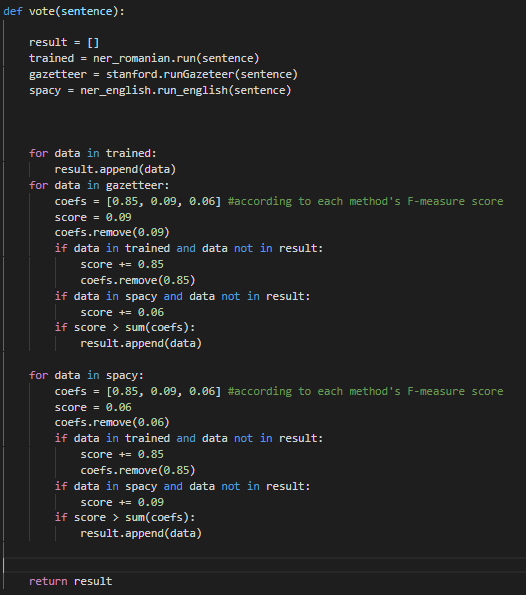
\includegraphics[scale = 0.55]{voting} }
\end{center}
\caption{The Python implementation of the voting function.}
\end{figure}

\begin{figure}[h!]
\begin{center}
  \makebox[\textwidth]{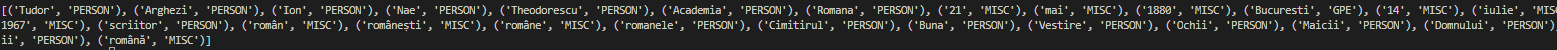
\includegraphics[width = \textwidth]{outputvoting} }
\end{center}
\caption{The output of the voting function.}
\end{figure}

\qquad Each classifier behaves differently with respect to each of the classes (meaning that one of them may be better with PERSON entities, one with GPE entities and so on). This suggests that for each of the identified entities one needs to combine the results of the three classifiers into one score.

\subsection{The Web Application}
\qquad \quad For the user interface, this thesis has adopted the use of a web application with a user-friendly front-end, as well as all the necessary information about the thesis. One can observe that a minimalist approach has been chosen, as depicted in Figure 30.

\begin{figure}[h!]
\begin{center}
  \makebox[\textwidth]{
\includegraphics[width = \textwidth]{site0} }
\end{center}
\caption{The homepage of the web application.}
\end{figure}

\qquad The operation of the aforementioned application is fairly simple, as the user has to input the sentence he wants to label, and the result of said classification will appear on the right side of the box, just as Figure 31 depicts.

\begin{figure}[h!]
\begin{center}
  \makebox[\textwidth]{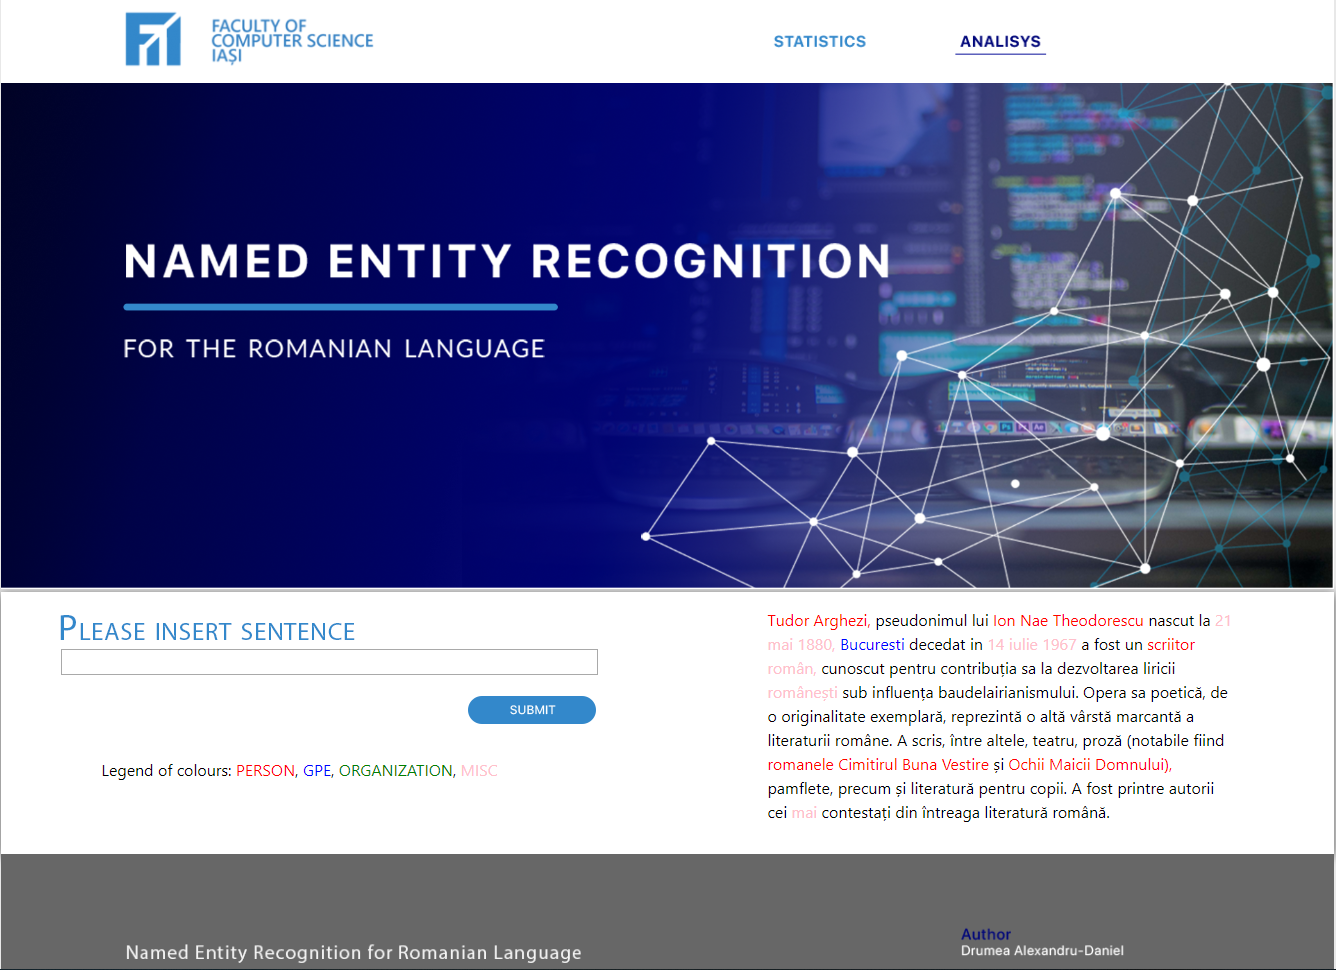
\includegraphics[width = \textwidth]{site} }
\end{center}
\caption{The homepage of the web application with labeled text.}
\end{figure}

\qquad The logic of this application is as follows, the user input is extracted from the front-end, it being passed on to the voting function described previously. The voting function will do the named entity recognition as described in the previous sections, then call the beautify function (Figure 32), which will return the newly
formed text, with the words labeled, using the colours described in the legend section of the page.

\qquad In order for all of the above to be fulfilled, Flask, the microframework described at Section 2.2 has been used, employing the same approach described in great detail there. 

\begin{figure}[h!]
\begin{center}
  \makebox[\textwidth]{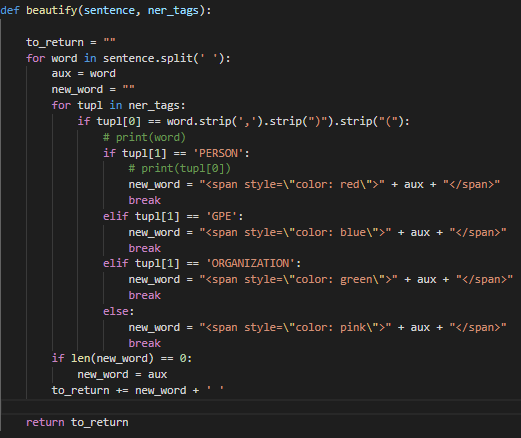
\includegraphics[width = \textwidth]{beautify} }
\end{center}
\caption{The beautify function.}
\end{figure}
\newpage
\section{Conclusions}
\qquad \quad The methods used in the current thesis have returned results that are satisfying as well as comprehensive. One has managed to achieve an F-measure score of 85$\%$, which consistently makes reliable classifications of sentences when it comes to named entities. If on a relatively short training data set the results have been such satisfying, one may assume that on a much more complex data set, the metrics will improve, the application having to reach a higher level of accuracy.

\qquad As one may have noticed in the course of this brief documentation, the premise of having a named entity recognizer has been achieved in a very comprehensive manner.

\qquad The first steps taken in the beginning of this thesis were to take the state of the art technologies such as SpaCy and test them on an unannotated, Romanian text. This procedure achieves an F-measure score of just 52$\%$, which despite not being satisfying, is not a negligible score either.

\qquad The Gazetteer method, which in some areas provide one with quite accurate classifications,  has its drawbacks, having achieved an F-measure score of 66$\%$,, which primarily comes from the difficulty of keeping a gazetteer up-to-date, as well as its lack of context awareness, thus making it not such a reliable, long-term tool.

\qquad The aim of this thesis has been reached by using the Conditional Random Field Algorithm of the Stanford Named Entity Recognition Software, which has obtained a score of 85$\%$ accuracy. Even though it is not quite at the level of the industry standard, it is a fine attempt in solving the problem of named entity recognition for the Romanian language.

\qquad Improvements are required in order for the application to become a reliable, powerful, industry standard tool, these improvements being: bigger contexts, more data, more ambiguity applied to said data, as well as much more powerful computers than the one used in the current thesis. 

\qquad In conclusion, the aim set at the beginning of this paper has been achieved, the knowledge gathered has been documented and the improvements needed have been identified and, therefore, the premises for further studies with more ambitious goals have been set.

\newpage
\section{Bibliography}
\begin {center}

\begin{enumerate}
\item Charles Sutton, Andrew McCallum (2011), "An Introduction to Conditional Random Fields", Vol. 4, No. 4, 267–373

\item Anca-Diana Bibiri, Mihaela Colhon, Paul Diac, Dan Cristea (2014). Statistics Over A Corpus Of Semantic Links: "QuoVadis". In Mihaela Colhon, Adrian Iftene, Verginica Barbu Mititelu, Dan Cristea, Dan Tufiş (eds.) (2014). Proceedings of the 10th International Conference "Linguistic Resources And Tools For Processing The Romanian Language, Craiova, 18-19 September 2014", "Alexandru Ioan Cuza" University Publishing House, pag. 33-44

\item Y. LeCun, L. Bottou, Y. Bengio and P. Haffner (November 1998), Gradient-Based Learning Applied to Document Recognition, Proceedings of the IEEE, 86(11):2278-2324

\item Wen-tau Yih, Xiaodong He, Christopher Meek (June 2014), Microsoft Research, Association for Computational Linguistics, "Semantic Parsing for Single-Relation Question Answering", 

\item Xiaodong Liu, Jianfeng Gao, Xiaodong He, Li Deng, Kevin Duh, Ye-Yi Wang (May 2015), NAACL, "Representation Learning Using Multi-Task Deep Neural Networks for Semantic Classification and Information Retrieval"

\item Nal Kalchbrenner, Edward Grefenstette, Phil Blunsom (2014), Department of Computer Science, "A Convolutional Neural Network for Modelling Sentences", University of Oxford

\item Ronan Collobert, Jason Weston, Leon Bottou, Michael Karlen, Koray Kavukcuoglu, Pavel Kuksa (2011), "Natural Language Processing (Almost) from Scratch", "Journal of Machine Learning Research 12"  2493-2537

\item https://github.com/dumitrescustefan/ronec

\item https://nlp.stanford.edu/software/CRF-NER.shtml

Cristea D., Gîfu D., Pistol I., Sfirnaciuc D., Niculiţă M. (2016) A Mixed Approach in Recognising Geographical Entities in Texts. In: Trandabăţ D., Gîfu D. (eds) Linguistic Linked Open Data. RUMOUR 2015. Communications in Computer and Information Science, vol 588. Springer, Cham
\item $https://spacy.io/models/xx$

\item $https://towardsdatascience.com/named-entity-recognition-with-nltk-and-spacy-8c4a7d88e7da$

\item $https://towardsdatascience.com/precision-vs-recall-386cf9f89488$

\item Charles Sutton, Andrew McCallum (2011), "An Introduction to Conditional Random Fields", Foundations and Trends in Machine Learning Vol. 4, No. 4, 267–373

\item Manning, Christopher D., Mihai Surdeanu, John Bauer, Jenny Finkel, Steven J. Bethard, and David McClosky (2014). The Stanford CoreNLP Natural Language Processing Toolkit In Proceedings of the 52nd Annual Meeting of the Association for Computational Linguistics: System Demonstrations, pp. 55-60.

\item https://blog.sicara.com/train-ner-model-with-nltk-stanford-tagger-english-french-german-6d90573a9486

\item https://profs.info.uaic.ro/~dcristea/papers/RUMOUR-Cristea$\%$20et$\%$20al.pdf

\item https://pythonprogramming.net/named-entity-recognition-nltk-python/

\item Manning, Christopher D. and  Surdeanu, Mihai  and  Bauer, John  and  Finkel, Jenny  and  Bethard, Steven J. and  McClosky (2014), "The Stanford CoreNLP Natural Language Processing Toolkit", Association for Computational Linguistics, 55-60

\item http://www.aclweb.org/anthology/P/P14/P14-5010

\item https://pythonhow.com/how-a-flask-app-works/

\item https://profs.info.uaic.ro/~dcristea/cursuri/IA/2018-2019\\/Curs13-$\%$20Analiza$\%$20limbajului$\%$20natural.ppt.pdf

\item https://developers.google.com/machine-learning/crash-course/classification/\\precision-and-recall

\item https://universaldependencies.org/

\item Doug Cutting and Julian Kupiec and Jan Pedersen and Penelope Sibun (1992) ,"A Practical Part-of-Speech Tagger", ANLC '92 Proceedings of the third conference on Applied natural language processing
Pages 133-140

\item https://medium.com/@jrodthoughts/ambiguity-in-natural-language-processing-15f3e4706a9a

\item https://www.quora.com/How-does-CNN-work-with-NLP

\item https://en.wikipedia.org/wiki/Convolutional$\_$neural$\_$network\\$\#$Natural$\_$language$\_$processing

\item http://flask.pocoo.org/

\item https://www.techopedia.com/definition/13825/named-entity-recognition-ner

\item https://medium.com/explore-artificial-intelligence/introduction-to-named-entity-recognition-eda8c97c2db1

\end{enumerate} 
\end{center}
\end{document}